\subsection{Umrechnung zwischen Dezimal und Dezibel}
    \begin{equation*}
        |\Sigma(s)|_{dB} = 20 \cdot \textrm{log}_{10}|\Sigma(s)| =             20\cdot\frac{\textrm{ln}(|\Sigma(s)|)}{\textrm{ln}(10)}
    \end{equation*}
    \begin{equation*}
        |\Sigma(s)| = 10^{\frac{|\Sigma(s)|_{dB}}{20}}
    \end{equation*}
    \begin{center}
    {\renewcommand{\arraystretch}{1.4}
        \begin{tabular}{c|c}
        Dezimalskala    &   Dezibelskala [dB]\\
        \hline
        100 &   40  \\
        10  &   20  \\
        5   &   13.97..\\
        3.16.. & 10\\
        2   &   6.02..\\
        1   &   0   \\
        $\frac{1}{\sqrt{2}}$  &   -3.0103\\
        0.5 & -6.02\\
        0.316.. & -10\\
        0.1 &   -20 \\
        0.01    &   -40\\
        0       &   $-\infty$
        \end{tabular}}
    \end{center}
    \begin{equation*}
        |\Sigma(j\omega)|_{dB} = |\Sigma_1(j\omega)|_{dB}+|\Sigma_2(j\omega)|_{dB}
    \end{equation*}
    \begin{equation*}
        \angle\Sigma= \angle\Sigma_{1}+ \angle\Sigma_{2}
    \end{equation*}
    \begin{equation*}
        \angle\Sigma(j\omega)=
        \begin{cases}
            \arctan(\frac{x}{y}) & x > 0\\
            \arctan(\frac{x}{y})+\pi & x<0
        \end{cases}
    \end{equation*}
    
\subsection{Übertragungsfunktionen}
    Matrix mit den herkömmlichen Übertragungsfunktionen.
    \begin{equation*}
        \begin{bmatrix}
            U(s)\\Y(s)\\E(s)
        \end{bmatrix}
        =
        \begin{bmatrix}
            S(s)    &   -S(s)\cdot C(s) &   S(s)\cdot C(s)\\
            S(s)\cdot P(s)  &   S(s)    &   T(s)\\
            -S(s)\cdot P(s) &   -S(s)   &   S(s)
        \end{bmatrix}
        \cdot
        \begin{bmatrix}
            W(s)\\D(s)\\R(s)
        \end{bmatrix}
    \end{equation*}
    
\subsection{Nyquist Theorem/Nominelles Stabilitätskriterium von Nyquist}
    Bestimmung der Stabilität von $T(s)$ durch $L(s)$ (ohne Modellunsicherheit).
            
    Der geschlossene Regelkreis mit Übertragungsfunktion $T(s)$ ist asymptotisch stabil, falls für $L(s)$ gilt:
        \begin{equation*}
            n_c\overset{!}{=}\frac{n_0}{2}+n_+
        \end{equation*}
        \begin{tabular}{l l}
            $n_c$:  & Anzahl Umrundungen um den kritischen Punkt (-1,0)  \\
                    & Positiv falls Umrundung gegen Uhrzeigersinn.\\
            $n_0$:  & Anzahl Pole von $L(s)$ mit Realteil = 0\\
            $n_+$:  & Anzahl Pole von $L(s)$ mit Realteil $>$ 0
        \end{tabular}
  
 \subsection{Beschränkung der Durchtrittsfrequenz}
    \begin{equation*}
        \boxed{\omega_c = 
        \begin{cases}
        \omega_c > \textrm{max}\{10\cdot\omega_d, 2\cdot\omega_{\pi^+}\}\\
        \omega_c < \textrm{min}\{\frac{1}{10}\cdot\omega_n, \frac{1}{10}\cdot \omega_2, \frac{1}{2}\cdot \omega_\tau, \frac{1}{2}\cdot \omega_{\zeta^+}\}
        \end{cases}
        }
    \end{equation*} 
    
\subsection{PID - Recap}
    Der PID-Regler hat folgende Form:
    \begin{equation*}
        C_{\textnormal{PID}}(s) = k_p\cdot\left(1 + \frac{1}{T_i\cdot s} + T_d\cdot s\right) = k_p\left(\frac{T_d\cdot T_i\cdot s^2 + T_i\cdot s + 1}{T_i\cdot s}\right)
    \end{equation*}
    
    \subsubsection{Ziegler-Nichols}
    \begin{equation*}
        P(s) \approx \frac{k}{\tau\cdot s + 1}\cdot e^{-T\cdot s}, \quad \frac{T}{T+\tau} < 0.3
    \end{equation*}
        \begin{equation*}
            \boxed{|k_p^* \cdot P(j\omega^*)| \overset{!}{=} 1} \hspace{3mm}
            \boxed{\angle k_p^* \cdot P(j\omega^*)\overset{!}{=}-\pi} \hspace{3mm}
            \boxed{T^* =\frac{2\pi}{\omega^*}}
        \end{equation*}
        \begin{center}
        {\renewcommand{\arraystretch}{1.2}
            \begin{tabular}{l r r r}
            Regler & $k_p$ & $T_i$ & $T_d$ \\
                 \hline
                P & $0.5\cdot k_p^*$ & $\infty \cdot T^*$ & $0 \cdot T^*$ \\
                PI & $0.45\cdot k_p^*$ & $0.85\cdot T^*$ & $0 \cdot T^*$\\
                PD & $0.55 \cdot k_p^* $& $\infty \cdot T^*$ &  $0.15\cdot T^*$\\
                PID & $0.6\cdot k_p^*$ & $0.5 \cdot T^*$ & $0.125 \cdot T^*$\\
            \end{tabular}}
        \end{center}

\subsection{Inverse einer 2x2-Matrix}
    \begin{equation*}
        A = \begin{bmatrix} a & b \\ c & d \end{bmatrix}\quad
        A^{-1} = \frac{1}{a\cdot d - c\cdot b}\begin{bmatrix} d & -b \\ -c & a \end{bmatrix}\quad
    \end{equation*}
    
\subsection{Nützliche Ableitungen}
    \begin{equation*}
        \frac{\partial}{\partial x}\arctan(ax) = \frac{a}{1+(ax)^2}
    \end{equation*}

\vfill\null\columnbreak
\subsection{Signalflussbilder}
    \begin{figure}[H]
        \centering
        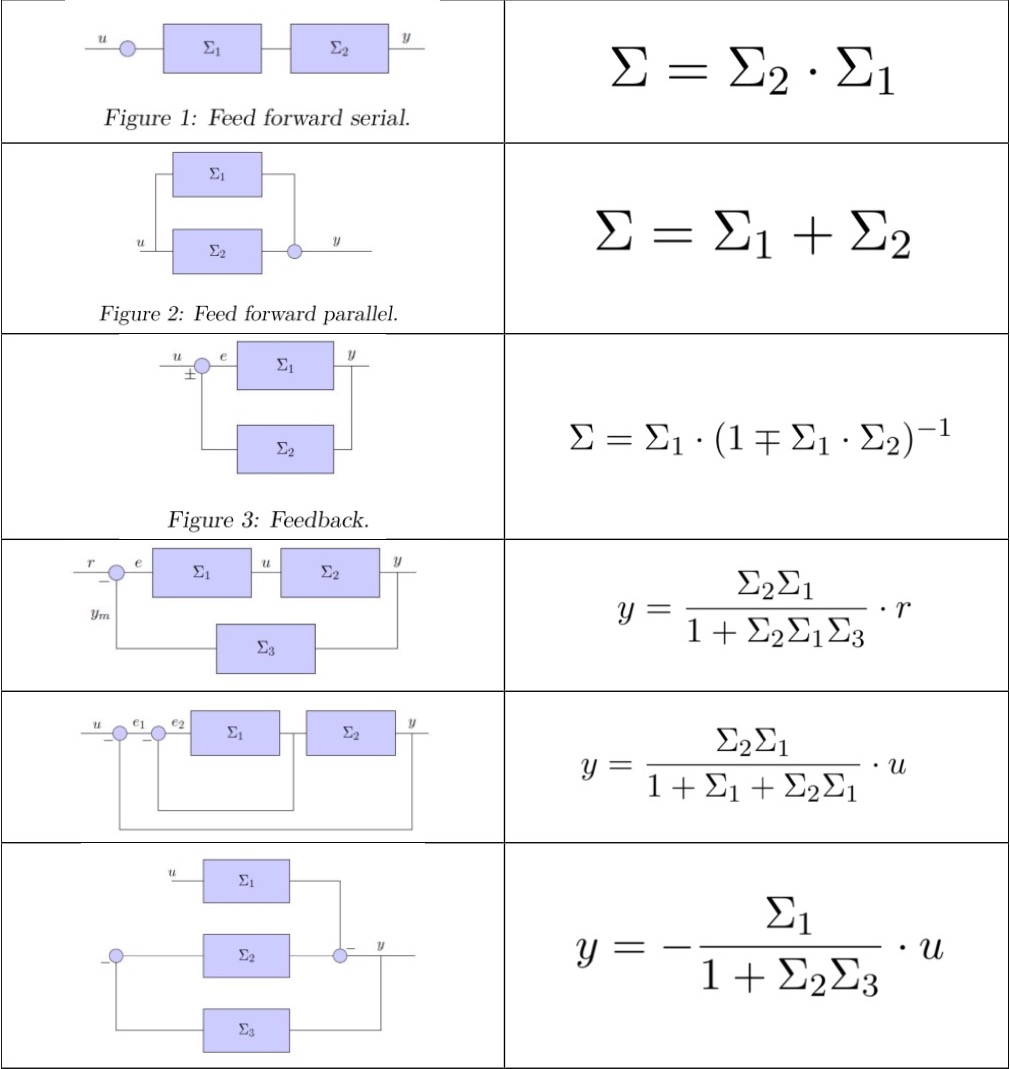
\includegraphics[width = 0.9\linewidth]{01/01_signalfluesse.jpg}
        \caption{Singalflussbilder und dazugehörige Transfer Functions.}
    \end{figure}